\section{Background on graphics processing units (GPUs)}

\begin{frame}[t]
\frametitle{Graphics processing units}
\begin{columns}[T]
\begin{column}{0.5\textwidth}
\begin{itemize}
\item Highly parallel and multi-threaded accelerator
    \begin{itemize}
        \item NVIDIA Tesla K20 accelerator: 2496 cores
        \item Focus on \emph{throughput}, not execution speed
    \end{itemize}
\item Spectacular performance for workloads that
    are compute-intensive, data-parallel
    (\emph{fine grained parallelism})
\item Effective use requires careful redesign
    of algorithms, code modification,
    and substantial tuning efforts
\item Vendors: NVIDIA, AMD
\end{itemize}
\end{column}
\begin{column}{0.5\textwidth}
\begin{figure}
\begin{center}
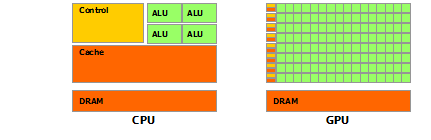
\includegraphics[width=150px]{img/device-comparison.png}
\caption{Design philosophies of CPU and GPU.\newline
Credit: NVIDIA CUDA programming guide}
\centering
\end{center}
\end{figure}
\end{column}
\end{columns}
\end{frame}

\begin{frame}
\frametitle{Performance considerations}
\begin{itemize}
\item CPU-GPU transfers expensive -
    hide communication cost by keeping GPU busy
\item Expose as much parallelism as possible
    to utilize GPU cores effectively
\item Avoid thread divergence and excessive
    synchronization
\item Memory access:
    \begin{itemize}
        \item Threads must access GPU memory (\emph{global} memory) in \emph{coalesced}
            fashion
        \item Threads must do enough work to hide
            memory access latency
    \end{itemize}
\item Strided or uncoalesced memory access patterns:
    use explicitly managed cache (\emph{shared} memory)
\end{itemize}
\end{frame}

